\section{Spurregler}

Um den Spurhalter zu verbessern, haben wir den bereits existierenden Regler optimiert.\\
Die Spurerkennung  lassen wir nun auf einem variablen Streifen des Bildes durchführen. Während die Breite des Streifens konstant ist, passt sich die Position an dem zuletzt gefundenen Straßenabschnitt an. Das Auto wird also dort nach der Straße suchen, wo vorher die Straße war. Außerdem lassen wir dunkle Grautöne in der Erkennung unberücksichtigt, sodass nur noch Kanten zu hellen Objekten gefunden werden.\\
Zusätzlich haben wir den maximal möglichen Lenkwinkel erhöht und berücksichtigen ihn, um die Geschwindigkeit des Autos zu verändern. 
Bei einem großen Winkel wird die Geschwindigkeit gedrosselt, während  die Geschwindigkeit erhöht wird, wenn der Winkel gering ist.
Dies resultiert in einer höheren Geschwindigkeit auf geraden Strecken.

%\begin{center}
%\resizebox{.9\textwidth}{!}{%
%\includegraphics[height=3cm]{Bildbild.jpg}%
%\caption{Text}
%\quad
%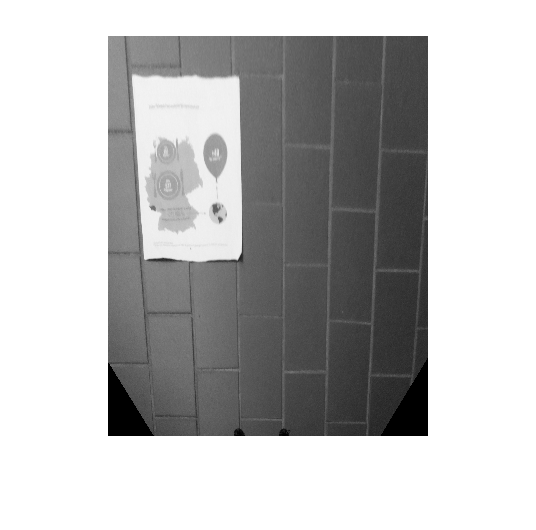
\includegraphics[height=3cm]{vogel2.png}%
%}
%\end{center}

